\chapter{Обзор и анализ различных систем обработки исключительных ситуаций} \label{ch2}
	
% не рекомендуется использовать отдельную section <<введение>> после лета 2020 года
%\section{Введение} \label{ch2:intro}

Данная глава посвящена разбору существующих проблем в системе обработок ошибок, предлагаемой кампанией Oracle. 

В параграфе \ref{ch2:sec2} рассматриваются разработки разных авторов, нацеленные на решение схожих проблем. 

Про то, как происходит работа с исключительными ситуациями рассказывается в параграфе \ref{ch2:sec3}.
В параграфе \ref{ch2:sec4} приведен краткий обзор механизма взаимодействия с ошибками в объектно-ориентированных языках, на примере C\#.

Описание функциональных возможностей, которые необходимы в разрабатываемом пакете, перечисляются в параграфе \ref{ch2:sec5}.



\section{Существующие проблемы обработки ошибок}\label{ch2:sec1}
Несмотря на то, что существующая система имеет довольно много возможностей для разработчиков, она не лишена недостатков. Далее будут рассмотрены некоторые проблемы, с которыми сталкиваются программисты при разработке программного обеспечения для базы данных.

Дублирование кода. Довольно часто встречаются ситуации, в которых возможно возникновение одних и тех же ошибок, для обработки которой придется воспроизводить уже написанный код. Дублирование кода противоречит принципу разработки программного обеспечения DRY (Don’t repeat yourself, рус. не повторяйся), предложенного Энди Хайдом и Дэйвом Томасом в книге «Программист-прагматик»\cite{pragmatic}. Увеличение кодовой базы приводит к увеличению затрат ресурсов при отладке и корректировки приложения. Одним из способов решения данной проблемы является вынесение повторяющегося кода в отдельные процедуры или функции, и заменой повторяющегося кода на вызов необходимых подпрограмм. 

Очень явно данная проблема выражена при работе с пакетом UTL\_FILE, а конкретнее, с процедурой GET\_LINE. Данная процедура предназначена для извлечения строк из файлов, и в случае невозможности считать новую строку, будет выдано исключение NO\_DATA\_FOUND. Это приводит нас к тому, что каждый раз, когда нам необходимо считать данные из файла, мы должно написать код для обработки этой ошибки, который будет везде одинаковый. Данный код будет затруднять понимание основной логики, а допущенная ошибка при копировании кода, может привести к нежелательным последствиям\cite{utl-file}. 

\begin{figure}[ht!] 
	\center
	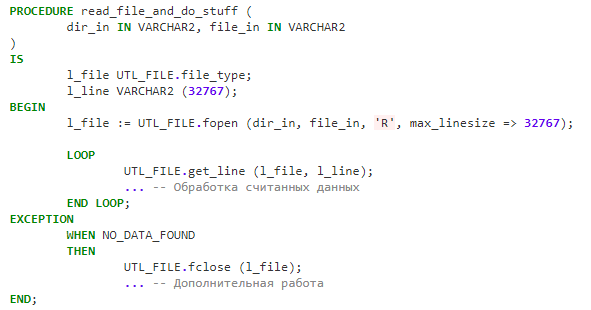
\includegraphics [scale=1] {my_folder/img/C1_utl_file_problem}
	\caption{Пример использования UTL\_FILE} 
	\label{fig:C1_utl_file_problem}  
\end{figure}
\FloatBarrier

На \firef{fig:C1_utl_file_problem} показан пример процедуры для чтения и обработки файла, с использованием пакета UTL\_FILE. Половину кода занимает обработчик ошибок, который должен присутствовать и обычно будет выполнять одну и ту же работу. Все это можно было бы сокрыть за одной функцией и работать с файлами при помощи вызова нужной подпрограммы, что займет всего одну строку кода, но позволит сократить количество ошибок и сэкономить время, затраченное на написание кода. В более сложных ситуациях, при которых использование процедуры такого вида невозможно по тем или иным причинам, все также можно будет воспользоваться пакетом UTL\_FILE.

Другой немаловажной проблемой при работе с ошибками является тот факт, что EXCEPTION в PL/SQL это особая разновидность структуры данных. Мы имеем достаточно небольшой набор возможностей для работы с ней, после объявления переменной данного типа, мы можем только инициировать или обрабатывать ее. Нету возможности для расширения функциональности данной структуры, мы не можем добавить дополнительные поля, мы не можем передавать исключения как параметр для процедуры или функции.

Также Oracle не дает возможностей для организации и классификации исключительных ситуаций, относящихся к конкретному приложению. В нашем распоряжении находиться 1000 кодов в диапазоне от -20999 до -20000. Разработчику необходимо следить чтобы коды использовались правильно, разные ошибки не должны связываться с одним и тем же кодом\cite{ferstein}. При боольшом количестве разработчиков это может быть затруднительно.

Для решения последних двух проблем можно реализовать альтернативную систему. Мы можем создать свои исключения и работать непосредственно с ними. Например, перечислить ошибки в отдельной таблице, тогда мы сможем передавать ошибки как параметры, дополнять всеми необходимыми для нас атрибутами, а необходимость контролировать это все перейдет от программиста к пакету, который будет этим заниматься. Под собственными ошибками будут скрыты исключения PL/SQL, в таком случае, мы, не потеряв преимуществ от работы со стандартных исключениями, будем иметь возможность при необходимости расширить их функциональность\cite{kite}. 

Дополнить такой пакет можно множеством различных способов, мы имеем полный контроль над аудитом ошибок, и можем его корректировать под свои нужды, в зависимости от приложения, можно собирать необходимый контекст возникновения ошибки и дополнять его при необходимости. Расширение пакета подпрограммами для обработки часто возникающих исключительных ситуаций позволит избежать проблемы дублирования кода. 


\section{Альтернативные возможности для обработки исключительных ситуаций}\label{ch2:sec2}

С обозначенными проблемами сталкивались и другие разработчики. Рассмотрим какие существуют способы улучшения процесса обработки ошибок. 

Стивен Ферштейн в своем докладе \cite{BestPracticePLSQL} про хорошие практики программирования на PL/SQL упоминает про Quest Error Manager (QEM). Получить много информации о нем не удалось, так как его перестали обновлять еще в 2010 году. Удалось выяснить, что этот довольно старый пакет, разработанный кампанией Quest, предназначался для решения схожих проблем. Установлено, что целью данного пакета было упрощение логирования информации об ошибках. 

В книге \cite{ferstein} Ферштейн и Прибыл выделяют похожие трудности при работе с исключительными ситуациями, и для изучения предоставляют пакет для обработки ошибок. Они говорят о том, что пакет не дописан и требует улучшений со стороны читателей, и предлагают выполнить это в качестве упражнения. Это небольшой пакет, состоящий всего из трех функций, предназначенный для демонстрации того, каким образом можно обрабатывать исключительные ситуации, альтернативным от стандартного способом. 

В ходе поиска существующих решений, было замечено, что во многих компаниях разрабатываются собственные пакеты для упрощения работы с обработчиками ошибок, но так как эти разработки являются собственностью кампаний, в открытом доступе их нет. 


\section{Механизмы обработки ошибок в других базах данных}\label{ch2:sec3}

Рассмотрим, как исключительные ситуации обрабатываются в других базах данных. 

В базе данных MySQL схема обработки ошибок довольно сильно схожа с той, которая применяется в Oracle Database. Здесь используются обработчики, которые, по своей сути, не отличаются от блока обработки ошибок в PL/SQL. Используется сигнальная схема, исключения именуются сигналами, тоже привязываются к кодам ошибок. Сигналы могут содержать дополнительную информацию об возникшей проблеме, которую можно указать при вызове сигнала, таковой информацией является: каталог, схема и имя ограничения, каталог, схема, колонка и название таблицы, имя курсора. 

Обработчики бывают разных типов, например, continue и exit. Они отличаются тем, что будет происходить, после того как сигнал обработается. 

В целом, такая система мало отличается от системы принятой в Oracle Database, и подвержена тем же проблемам, но имеет ряд возможностей упрощающих работу с ошибками и ускоряющих процесс написания кода\cite{MySqlDocumentation}.

Процедурный язык Transact-SQL, являющийся расширением языка SQL, разрабатывается кампанией Microsoft. Данный язык используется в базах данных SQL Server и Sybase.
В Transact-SQL исключительные ситуации обрабатываются посредством блока TRY…CATCH. Вызов ошибок происходит посредством команды RAISERROR, в которую передаются системные параметры ошибки, такие как код, сообщение, важность и положение.  Последний параметр позволяет конкретизировать место возникновение ошибки, если возникло несколько одинаковых ошибок в разных местах\cite{TSQLDocumentation}.

В базе данных PostgreSQL то, как вы будете обрабатывать ошибки, зависит от используемого языка процедурного расширения. Согласно документации, PL/pgSQL очень схож с процедурным языком Oracle PLSQl\cite{PostgreSqlDocumentation}.

Действительно, синтаксис работы с ошибками, мало отличается. Используются такие же конструкции для блока обработки, обращаться к ошибкам можно по имени или коду. Можно получать расширенную информацию об ошибке, схожую с информацией, передаваемой с событиями в MySQL. 

В общем, обработка исключений работает схоже в разных базах данных. Везде имеется завязка на коды ошибок, корректную работу с которыми должен контролировать программист. Расширение объектов типа EXCEPTION ограничено или вовсе отсутствует. 

\section{Примеры обработки ошибок в объектно-ориентированных языках}\label{ch2:sec4}

Рассмотрим, как происходит работа с исключительными ситуациями в других языках программирования. Рассматривать будем язык C\#. Изучим пример, приведенный на рисунке \ref{fig:C2_c_sharp_user_defined_exceptions}. 

\begin{figure}[ht!] 
	\center
	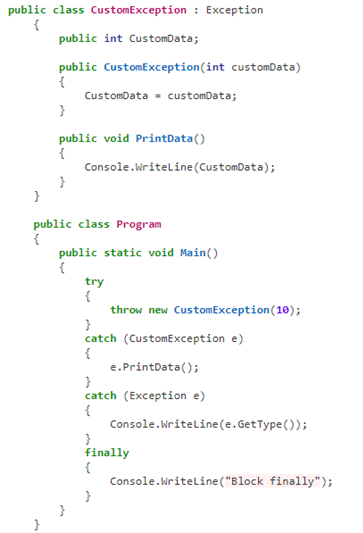
\includegraphics [scale=1] {my_folder/img/C2_c_sharp_user_defined_exceptions}
	\caption{Пример обработки ошибок в C\#} 
	\label{fig:C2_c_sharp_user_defined_exceptions}  
\end{figure}
\FloatBarrier

В данном коде объявляется пользовательская исключительная ситуация CustomException, она наследуется от базового класса Exception. В данном объекте мы объявляем переменную CustomData для хранения необходимой информации, а также метод PrintData, для вывода данной информации в консоль. 

Далее, в классе Program, в методе Main, происходит основная работа программы. Блок try/catch позволяет выполнить код, и в случае возникновения ошибки обработать ее. Мы имеем возможность выполнить различный код, в зависимости от ошибки, указывая несколько блоков catch (схожим образом мы разделяем обработку разных ошибок в PL/SQL). Аналогом блока try/catch в PL/SQL будет являться объявление вложенного блока begin/end с указанием ключевого слова exception. 

В коде, расположенном в блоке try создается экземпляр класса пользовательской ошибки, с указанием конкретных данных, в данном случае числа 10, и происходит вызов данного исключения, при помощи ключевого слова throw. В операторе catch выполняется обработка данной ошибки, вызывается созданный нами метод, который выведет информацию на консоль. 

Также, в данном примере, используется ключевое слово finally. Код, расположенный в данном блоке, выполнится независимо от того возникло какое-либо исключение или нет. Данная функциональность обычно используется для корректного завершения работы кода из блока try, например, для закрытия файлов, которые были ранее открыты.

В результате выполнения данного примера, на консоль будет выведенно две строки, первая, с числом 10, и вторая со строкой "Block finally".

Данный подход к работе с исключительными ситуациями не накладывает на нас ограничений, которые существуют в PL/SQL. Программисту не нужно следить за кодами ошибок, имеется достаточное количество предопределенных классов, с различными ошибками, мы можем спокойно передавать любое количество данных. Современные IDE подскажут разработчику какие исключения созданы, и уже из представленного списка, можно будет выбрать подходящее.

В других объектно-ориентированных языках взаимодействие с исключительными ситуациями происходит схожим образом. 


\section{Требования к разрабатываемому пакету}\label{ch2:sec5}

Среди выдвинутых проблем при обработке ошибок, особенно выделяется неудобство взаимодействия с кодами ошибок. Разработчики продукта обязаны самостоятельно контролировать и следить за тем, какие коды использованы, какие свободны, какой номер ошибки нужно применить в той или иной ситуации. Не редко для этих целей используется документ, в котором программисты составляют перечень номеров, которые уже используются. 
Для решения этой проблемы в пакете будет присутствовать таблица, содержащая подробную информацию об каждой ошибке. В которую входит: код ошибки, тип ошибки, имя для исключения, подробное описание исключительной ситуации, информация об области применения, дополнительная информация, специфичная для пользователей пакета. 

Особенно важной функциональностью для такого пакета является функциональность сохранения информации об возникающих ошибках. А также различные представления, предоставляющие удобный способ для анализа ошибок. Должна быть собрана информация об частотности возникновения ошибок, местах их появления, данных, которые привели к возникновению ошибке такого рода. 

Для избавления проблем с дублированием кода, будут предусмотрены несколько стандартных методов-обработчиков ошибок, с возможностью расширить тот список пользовательскими обработчиками. Среди стандартных обработчиков должны присутствовать:

\begin{enumerate}
\item Обработчик с логированием и повторным возбуждением исключения, заносящий информацию в специальное место, и передающий ошибку в вызывающий блок. 
\item Обработчик с логированием и сокрытием ошибки, данный метод будет сохранять информацию и завершать выполнение блока, в котором возникло исключение, без передачи ошибки дальше. 
\item «Тихие» обработчики, данные обработчики схожи по функционалу с предыдущими, но не производят логирования об возникшей ошибке. 
\item Обработчик критических ошибок, такой метод предназначен для работы с особо важными ошибками, затрагивающими основную логику приложения. Помимо занесения информации в стандартные места, данная процедура позволит сообщить администратору об возникновении критической ситуации, через другие каналы связи, например по почте. Функционал для настройки оповещения будет предусмотрен в разрабатываемом пакете. 
\end{enumerate} 


Необходима возможность для настройки параметров пакета, так называемые feature flag. Это поля (обычно содержащие бинарное значение), позволяющие включить или отключить, ту или иную функциональность. 

Данный список требований будет пополнен функциональными возможностями, необходимость в которых возникнет в ходе разработки.

\section{Выводы} \label{ch2:conclusion}
В ходе данной главы были рассмотрены проблемы, которые затрудняют разработку продуктов на языке Oracle PL/SQL. Были предложены различные способы для их устранения.
Был проведен разбор пакетов, упрощающих работу с исключительными ситуациями. Также было рассмотрено как обработка ошибок реализована в других СУБД. 
После этого были выдвинуты требования к реализуемому пакету, с описанием того, как та или иная функциональность способствует решению обозначенных проблем. 




%% Вспомогательные команды - Additional commands
%
\newpage % принудительное начало с новой страницы, использовать только в конце раздела
%\clearpage % осуществляется пакетом <<placeins>> в пределах секций
%\newpage\leavevmode\thispagestyle{empty}\newpage % 100 % начало новой страницы